% !TeX spellcheck = en_US
% !TeX encoding = UTF-8
% !TeX root = ../report.tex

\chapter{Introduction}
\label{chp:introduction}

The purpose of this chapter is to provide a contextual foundation for the topics discussed in the report, and to articulate the goals and motivation behind the thesis. Furthermore, the current state of research is explored, highlighting the key contributions and challenges that have shaped the direction of the work or provided ideas for further improvements. Lastly, an overview of the structure of the report is presented, allowing a better understanding of the organization and flow of the content.

\section{Context}
\subsection{Bridgestone World Solar Challenge}
\label{sec:BWSC}

Every two, universities from around the globe gather in Australia to participate in the world-renowned Bridgestone World Solar Challenge (BWSC)~\cite{BridgestoneWorldSolarChallenge:2022webpage}. After months of tireless preparation, these teams unveil their unique solar cars in Darwin, the starting point of the competition. Here, the cars are thoroughly inspected by judges to ensure they meet all necessary safety and performance standards. Once the starting order from the qualification is set, the teams are ready to embark on their journey across the Australian inland. The race spans approximately 3000 km and includes nine control stops along the route, as depicted in \cref{fig:RouteMap}.
\begin{figure}[htbp]
	\centering
	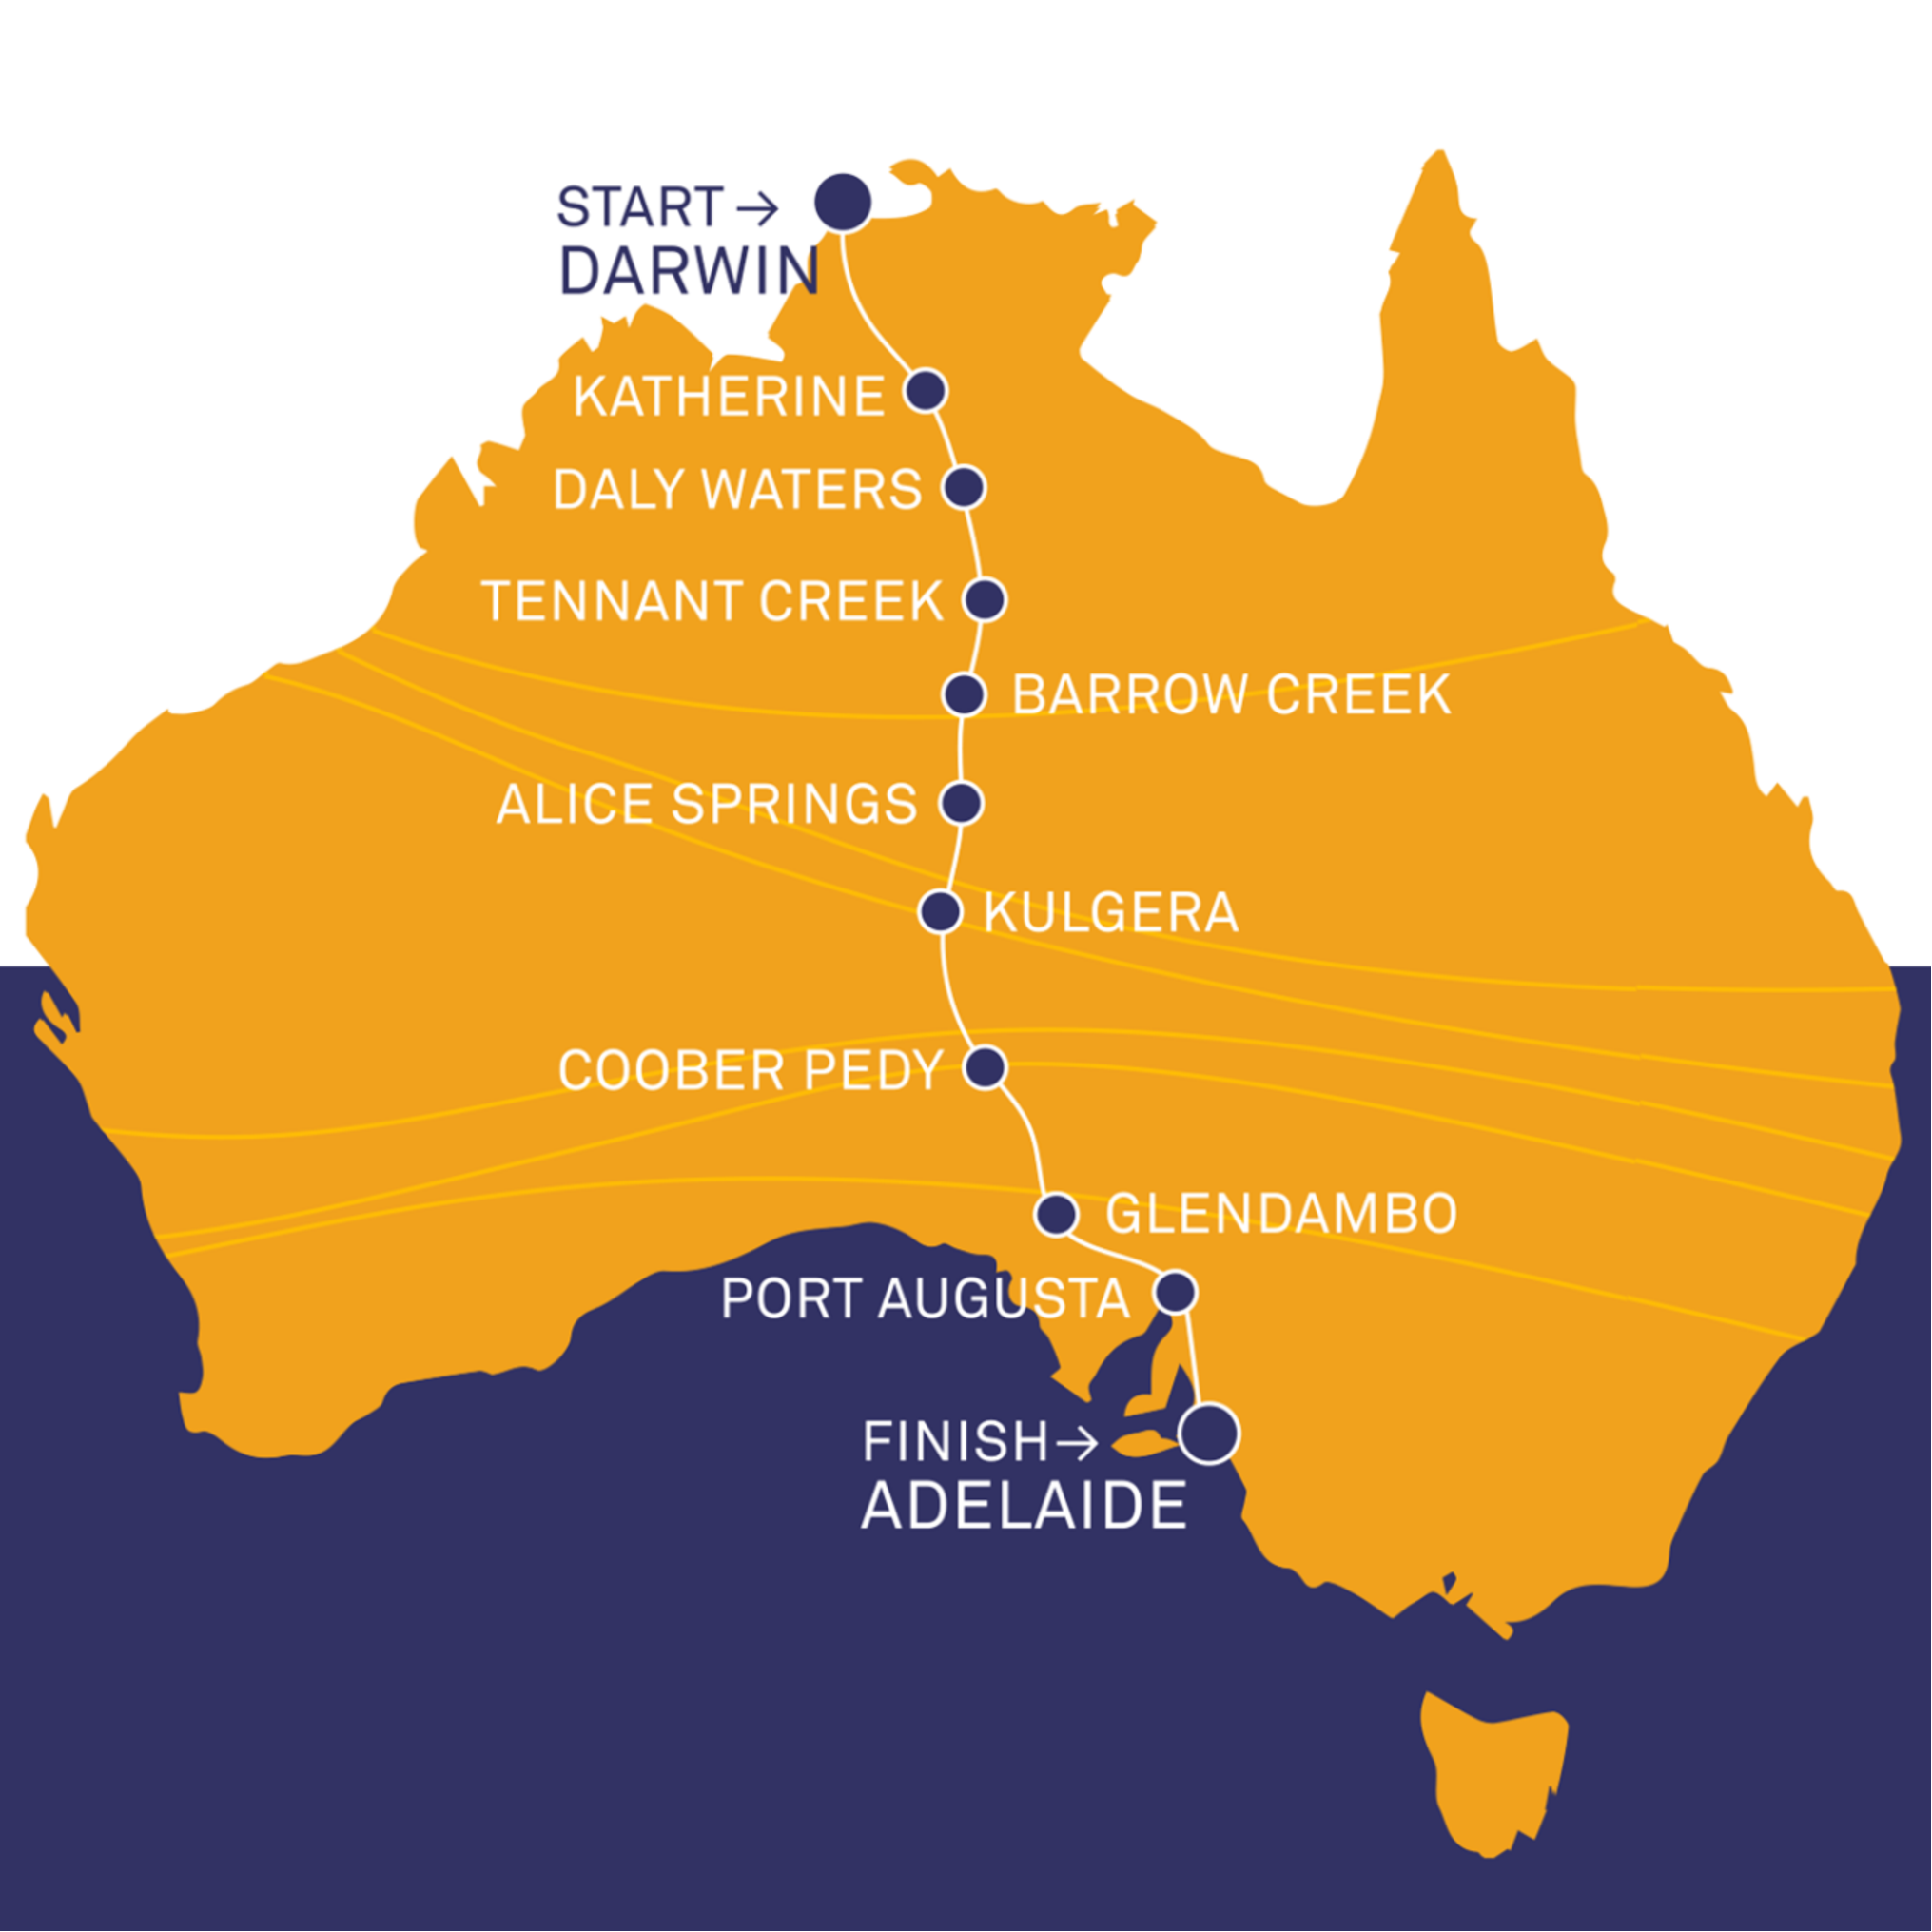
\includegraphics[width=0.5\textwidth]{img/RouteMap.pdf}
	\caption{Route map of the BWSC competition in Australia with the starting point in Darwin, the finish line in Adelaide, and the city names of the nine control stops~\cite{BridgestoneWorldSolarChallenge:2022webpage}.}
	\label{fig:RouteMap}
\end{figure}

The objective of each team is to build a car to be able to traverse the Australian desert as quickly as possible and be the first to cross the finish line~\cite{onTheSubjectOfSolarVehicles:2007}.


\subsection{Alpha Centauri Team}
The Mechanical Engineering Department (D-MAVT) and the Electrical Engineering Department (D-ITET) at ETH annually offer third-year undergraduate students the chance to conduct a \enquote{Fokus Projekt}. These projects encompass a variety of specializations and can be proposed by students or Professors. In 2022, a proposal by five students to construct a solar car for the \enquote{Challenger Class} of the BWSC was accepted, and the focus students were chosen.

The students then established the \textit{Alpha Centauri} association~\cite{alphaCentauri:2022webpage}, which now consists of over thirty members. In addition to the focus students, there are numerous students who contribute their time and expertise either freely or by writing their theses. The \textit{Alpha Centauri} team is composed of six interconnected sub-teams, each responsible for specific technical tasks, and an organizational board. This thesis is a part of the \enquote{Simulation and Strategy} sub-team, but is naturally related to other sub-teams as well.


\section{Motivation}
Over the past decade, the automotive industry has turned its attention to electric cars as a more sustainable and efficient alternative to vehicles powered by fossil fuels. This shift has been driven by concerns about pollution from internal combustion engines and the dangers associated with our reliance on fossil energy resources. In response, some companies are exploring the use of photovoltaic (PV) panels placed on top of electric vehicles~\cite{lightyear:2022webpage, sion:2022webpage, Fraunhofer:2022webpage}. This technological advancement does not only represent a significant step towards sustainable mobility, but has also the potential to improve the range of electric vehicles, making transportation more efficient and increasing consumer interest.

Before the development of these innovative technologies, solar cars were predominantly featured in competitions like the one described in~\cref{sec:BWSC}. These competitions serve as a platform to demonstrate the potential of solar cars as a solution to the aforementioned issues and also encourage innovation.

%Participating in such projects also offers an invaluable opportunity to learn and work in a team setting, and provides a perfect environment to apply the knowledge gained at university. I believe that this type of hands-on experience is crucial in any academic career.
 

\section{Objective}
The primary objective of this thesis is to use Simulink simulation as a tool to evaluate and refine the proposed strategy. Through simulation, various scenarios can be tested, hence assessing the sensitivity of key design parameters, and allowing the evaluation of performance of the solar car under different weather conditions.

The second objective is to determine an optimal state-of-charge reference profile that maximizes the utilization of available energy while also complying with physical constraints, such as component limitation in the battery and motor. This profile can then be used as reference for controllers in a simulation or during the competition.


\section{State of the Research}
Although many teams participate to the competition every two years, only few of their reports are made available to the public. This is often due to the competitive spirit of each team and the need to keep winning innovation secret from opponents.


\subsection{Modeling}
Many studies presented in the literature utilize similar modeling components and vehicle dynamics equations as originally presented in~\cite{winningSolarCar2003book}. However, there are also a number of reports that present distinct models, as listed here:
\begin{itemize}
	\item In~\cite{SolUTra:2006mt}, an air density model as function of the ambient temperature and altitude is derived. In addition to this, the efficiency of maximum power point tracking (MPPT) device is modeled. It usage is important because it adjusts the current or voltage generated by solar panels with the goal of maximizing the electrical power.
	\item The solar panel model in~\cite{optimalEnergyManagement:2000book} is particularly detailed, as it accounts for diffusive, direct, and reflected irradiance, as well as the curvature and inclination of the panels with respect to the zenith. It also includes electrochemical and heuristic models of the battery. However, the authors conclude that a simpler model is precise enough for the purposes of this competition.
\end{itemize}


\subsection{Optimization of the Race Strategy}
When considering optimization problems, it is possible to distinguish between online and offline approaches. Online optimization utilizes continuously gathered information during the race and includes updated weather forecasts. On the other hand, offline optimization focuses on finding a profile that optimizes a function or variable prior to the competition. The optimization problem of this thesis belongs to the offline category. Therefore, the relevant literature reports are presented for this category.

When discussing the strategy, it is more convenient to divide it into three categories based on the time horizon they cover: long-term, mid-term, and short-term~\cite{SolUTra:2006mt}.

\paragraph{Long-Term}
A long-term strategy encompasses an approach that considers the whole race horizon, as for the following reports.
\begin{itemize}
	\item Dynamic programming is a useful technique that allows for the insertion of stochastic weather forecasts and guarantees the attainment of a global optimum. It has been employed in the context of finding optimal driving behavior, as demonstrated in~\cite{racingWithTheSun:1997}.
	\item In~\cite{optimalEnergyManagement:2000book}, the author formulate the problem as a minimum time Meyer problem where the optimal solution is found by maximizing the Hamiltonian.
	\item The authors of~\cite{strategyOptimizationOfSolarCar:2013} propose an unique algorithm that works by iteratively improving a solution through a process of expansion (Big Bang) and contraction (Big Crunch). It operates on eleven segments, which represent different segments of the route, with the goal of finding the combination of segment-constant velocity that will minimize the driving time. The algorithm takes into account three possible weather scenarios.
	\item The authors of~\cite{heuristicOptimizationForTheEnergyManagement:2017article} compare various long-term optimization methods and concludes that non-constant velocity approaches tend to perform better. Two simplified weather scenarios are tested.
\end{itemize}
\paragraph{Mid-Term}
Day-by-day decisions are taken using mid-term strategy that are strongly affected by the weather, acceleration, and deceleration.
\begin{itemize}
	\item In~\cite{criticalSpeedControl:2002article}, an alternative to the constant-velocity approach is presented, in which the critical speed is determined as a function of solar irradiance.
\end{itemize}
\paragraph{Short-Term}
Short-term strategy refers to the approach taken for managing events that have a shorter duration, such as navigating turns, climbing hills, or dealing with unexpected occurrences like traffic jams and strong winds.
\begin{itemize}
	\item In~\cite{racingWithTheSun:1997}, the authors investigate short-term strategies for optimizing acceleration and deceleration in various driving scenarios, including approaching or leaving stops and hills.
\end{itemize}


\section{Structure of the Report}
\Cref{chp:introduction} contextualizes the topics of this thesis and provides an outline of the goals and motivation.

\Cref{chp:modeling} contains all the important modeling equations necessary to subsequently construct a simulation. Furthermore, it includes an analysis of the road and weather data.

\Cref{chp:simulation,chp:strategy} represent the heart of the report. First, in~\cref{chp:simulation} the Simulink simulation is thoroughly explained in all its parts, using simplified representations of block structures. Second, a racing strategy is proposed. In~\cref{chp:strategy} are presented the analytical and graphical methods used to obtain the reference profile.

\Cref{chp:results} contains the relevant quantitative results and a discussion thereof. A sensitivity analysis is also presented at the end of the chapter.

Lastly,~\cref{chp:conclusion} presents the final conclusion of the work, identifies opportunities for improvement, and discusses possible outlook.